
\section{Parte Informativa}
\subsection{Datos del practicante}
\begin{table}[h]
    \begin{tabular}{p{5cm} p{7cm} }
        Apellidos y nombres &: David Brahyan Larota Pilco  \\ 
        Código              &: 20816   \\ 
        Especialidad de prácticas    &: Ingeniería de software  \\ 
        Modalidad de prácticas    &: Presencial  \\ 
        Facultad    &: FIMEES  \\ 
        Promoción    &: 2025  \\ 
    \end{tabular}
\end{table}
\subsection{Centro de practicas}
\begin{table}[h]
    \begin{tabular}{p{5cm} p{10cm} }
        Nombre de la entidad &: Dirección de proyección social y extensión cultural \\ 
        Dependencia/Oficina              &: Oficina de dirección principal   \\ 
        Jefe inmediato    &: Dra. Milder Zanabria Ortega  \\ 
        Modalidad de prácticas    &: Presencial  \\ 
    \end{tabular}
\end{table}
\subsection{Periodo de prácticas}
\begin{table}[h]
    \begin{tabular}{p{5cm} p{10cm} }
        Fecha de inicio &: 15/04/2025  \\ 
        Fecha de Culminación              &: 15/07/2025    \\ 
        Duración    &: 3 Meses  \\ 
    \end{tabular}
\end{table}
\subsection{Docente de prácticas}
Dr. Pedro Feder Ponce Cordero

\newpage
\section{Introducción}
Las prácticas preprofesionales realizadas en la Oficina de Proyección Social y Extensión Cultural tienen como objetivo desarrollar habilidades en el análisis y desarrollo de software, aplicando los conocimientos adquiridos a lo largo de la carrera en un entorno profesional. Durante este periodo, he tenido la oportunidad de participar en diversas
actividades relacionadas con el desarrollo de soluciones tecnológicas para mejorar la gestión interna de la institución. 

\section{Obetivos de las prácticas pre profesionales}
\subsection{Obetivo general}
Desarrollar habilidades en el análisis, diseño y desarrollo de software en un entorno profesional, contribuyendo al avance de los proyectos de la Oficina de Proyección Social y Extensión Cultural.

\subsection{Obetivos específicos}
\begin{enumerate}
    \item Analizar y diseñar: el sistema que abarca tres subunidades (Proyección Social y Extensión Universitaria, Seguimiento y Desarrollo del Graduado, Gestión Ambiental).
    \item Desarrollar interfaces del software en función de las necesidades de la institución.
    \item Colaborar en la implementación de un módulo del sistema que optimice los procesos internos de gestión para sus proyectos que manejan.
    
\end{enumerate}

\section{Descripción del centro de prácticas}
\subsection{Nombre de la institución}
Oficina: Dirección de Proyección Social y Extensión Cultural

\subsection{Dirección del centro de prácticas}
Auditorio Mango UNA Puno (Tercer piso)

\subsection{Teléfono, fax, página web, correo electrónico}
\href{https://proyeccionsocial.com/}{https://proyeccionsocial.com/}

\begin{table}[h]
    \begin{tabular}{p{5cm} p{10cm} }
        +51 971710338 &: Ing Melissa (Encargada del proyecto).\\
        +51 951522828 &: Dra. Milder (Directora de la oficina DPSEC).\\
        +51 950036674 &: Oficina DPSEC (secretaria)
        
    \end{tabular}
\end{table}

\subsection{Visión}	
La Dirección de Proyección Social y Extensión Cultural fortalece el desarrollo de la región, bajo los principios de la ciencia, la tecnología, los valores culturales y la investigación en el marco de una responsabilidad social sostenible.

\subsection{Misión}
La Dirección de Proyección Social y Extensión Cultural es generadora de la interacción con la comunidad para el desarrollo regional a través de la ciencia, la tecnología y las expresiones culturales como parte de la labor académica y de investigación en el marco de la proyección social y extensión cultural sostenible.

\subsection{Valores institucionales}
\begin{enumerate}
    \item \textbf{Responsabilidad:} Compromiso con el cumplimiento de las obligaciones y tareas asignadas.
    \item \textbf{Respeto:} Reconocimiento y consideración hacia las personas, sus ideas y derechos.
    \item \textbf{Integridad:} Actuar con honestidad y ética en todas las acciones.
    \item \textbf{Compromiso Social:} Participación activa en el desarrollo y bienestar de la comunidad.
    \item \textbf{Excelencia:} Búsqueda constante de la calidad en el desempeño académico y profesional.
    
\end{enumerate}

\subsection{Objetivos de la institución}
Promover, organizar, dirigir, supervisar y evaluar las actividades en el marco de la proyección social, extensión cultural y dimensión ambiental sostenible de la universidad, orientados hacia la comunidad, con el fin de coadyuvar al desarrollo e inserción laboral, re-valorando su identidad cultural.

\subsection{Actividad principal de la institución}
La Dirección de Proyección Social y Extensión Cultural, es un órgano dependiente del Vicerrectorado Académico, responsable de promover, organizar, dirigir y supervisar las actividades en el marco del desarrollo sostenible de Proyección Social y Extensión Cultural de la universidad, orientados hacia la comunidad, con el fin de coadyuvar al desarrollo de la región, revalorando la identidad cultural.


\subsection{Funciones de la oficina de prácticas}
\begin{enumerate}
    \item Proponer reglamentos o directivas de su competencia, para aprobación y aplicación.
    \item Revalorar, promover y preservar la riqueza cultural de la región.   
    \item Promover y apoyar a los estudiantes en sus actividades culturales.	
    \item Vincular la universidad con la sociedad a través de actividades de extensión cultural y proyección social.
    \item Programar, organizar y ejecutar eventos científicos, tecnológicos y culturales que contribuyan al desarrollo de la región.
    \item Coordinar, ejecutar y supervisar los programas y proyectos de proyección social y extensión cultural universitaria.
    \item Establecer la racionalidad de la calendarización de las actividades culturales y deportivas de manera que no afecten el desarrollo de las actividades académicas.
    \item Proponer la política, objetivos, acciones estratégicas de Proyección Social y Extensión Cultural de la Universidad, en coordinación con las unidades orgánicas de la universidad.
    \item Diseñar y ejecutar planes, programas, estrategias y acciones para consolidar la vinculación y el soporte necesario para los graduandos de la UNA-PUNO.
    \item Desarrollar programas de apoyo en coordinación con las facultades a través de la extensión cultural y proyección social que permitan proponer soluciones viables y sustentables a problemas de la región.
    \item Realizar investigaciones relacionadas con la situación profesional, académica y laboral de los exalumnos de la universidad y de la relación entre el empleo y la oferta académica en su zona de influencia.
    \item Planificar, dirigir, ejecutar, supervisar y evaluar las actividades de mantenimiento de infraestructura ambiental, manejo adecuado de residuos, sensibilización y educación ambiental en la Universidad.
    \item Contribuir en la formulación de la política académica de la Universidad en materia de promoción y fomento del desarrollo sostenible, gestión de riesgos y adaptación al cambio climático y protección y conservación del medio ambiente.
    \item Registrar y administrar información y estadísticas de los graduados de la universidad, a través de un sistema informático integral, que permita procesar y obtener del mismo, una serie de reportes a fines a esta área para la toma de decisiones y la elaboración de planes de mejora.
    \item Proponer la suscripción de convenios de proyección social y extensión cultural de facultades con instituciones públicas, privadas y organizaciones de base, con la finalidad de objetivar los diferentes planes de desarrollo de estas organizaciones.
    \item Fomentar y promover la educación ambiental, participación en programas de gestión ambiental, proyectos de desarrollo y conservación del medio ambiente en todos los niveles dentro y fuera de la Universidad.
    \item Formular y proponer la aplicación de normas ambientales que promuevan la conservación del medio ambiente y adaptación al cambio climático en las actividades bajo la competencia de la Universidad.
    \item Las demás que le asigne el Vicerrectorado Académico o la Alta Dirección en el ámbito de su competencia.
    
\end{enumerate}

\subsection{Funciones específicas del practicante}


\subsection{Organigrama de la institución}
\begin{figure}[h] % Entorno para manejar imágenes
    \centering % Centra la imagen
    \caption{Organigrama de la institución} % Pie de la imagen
    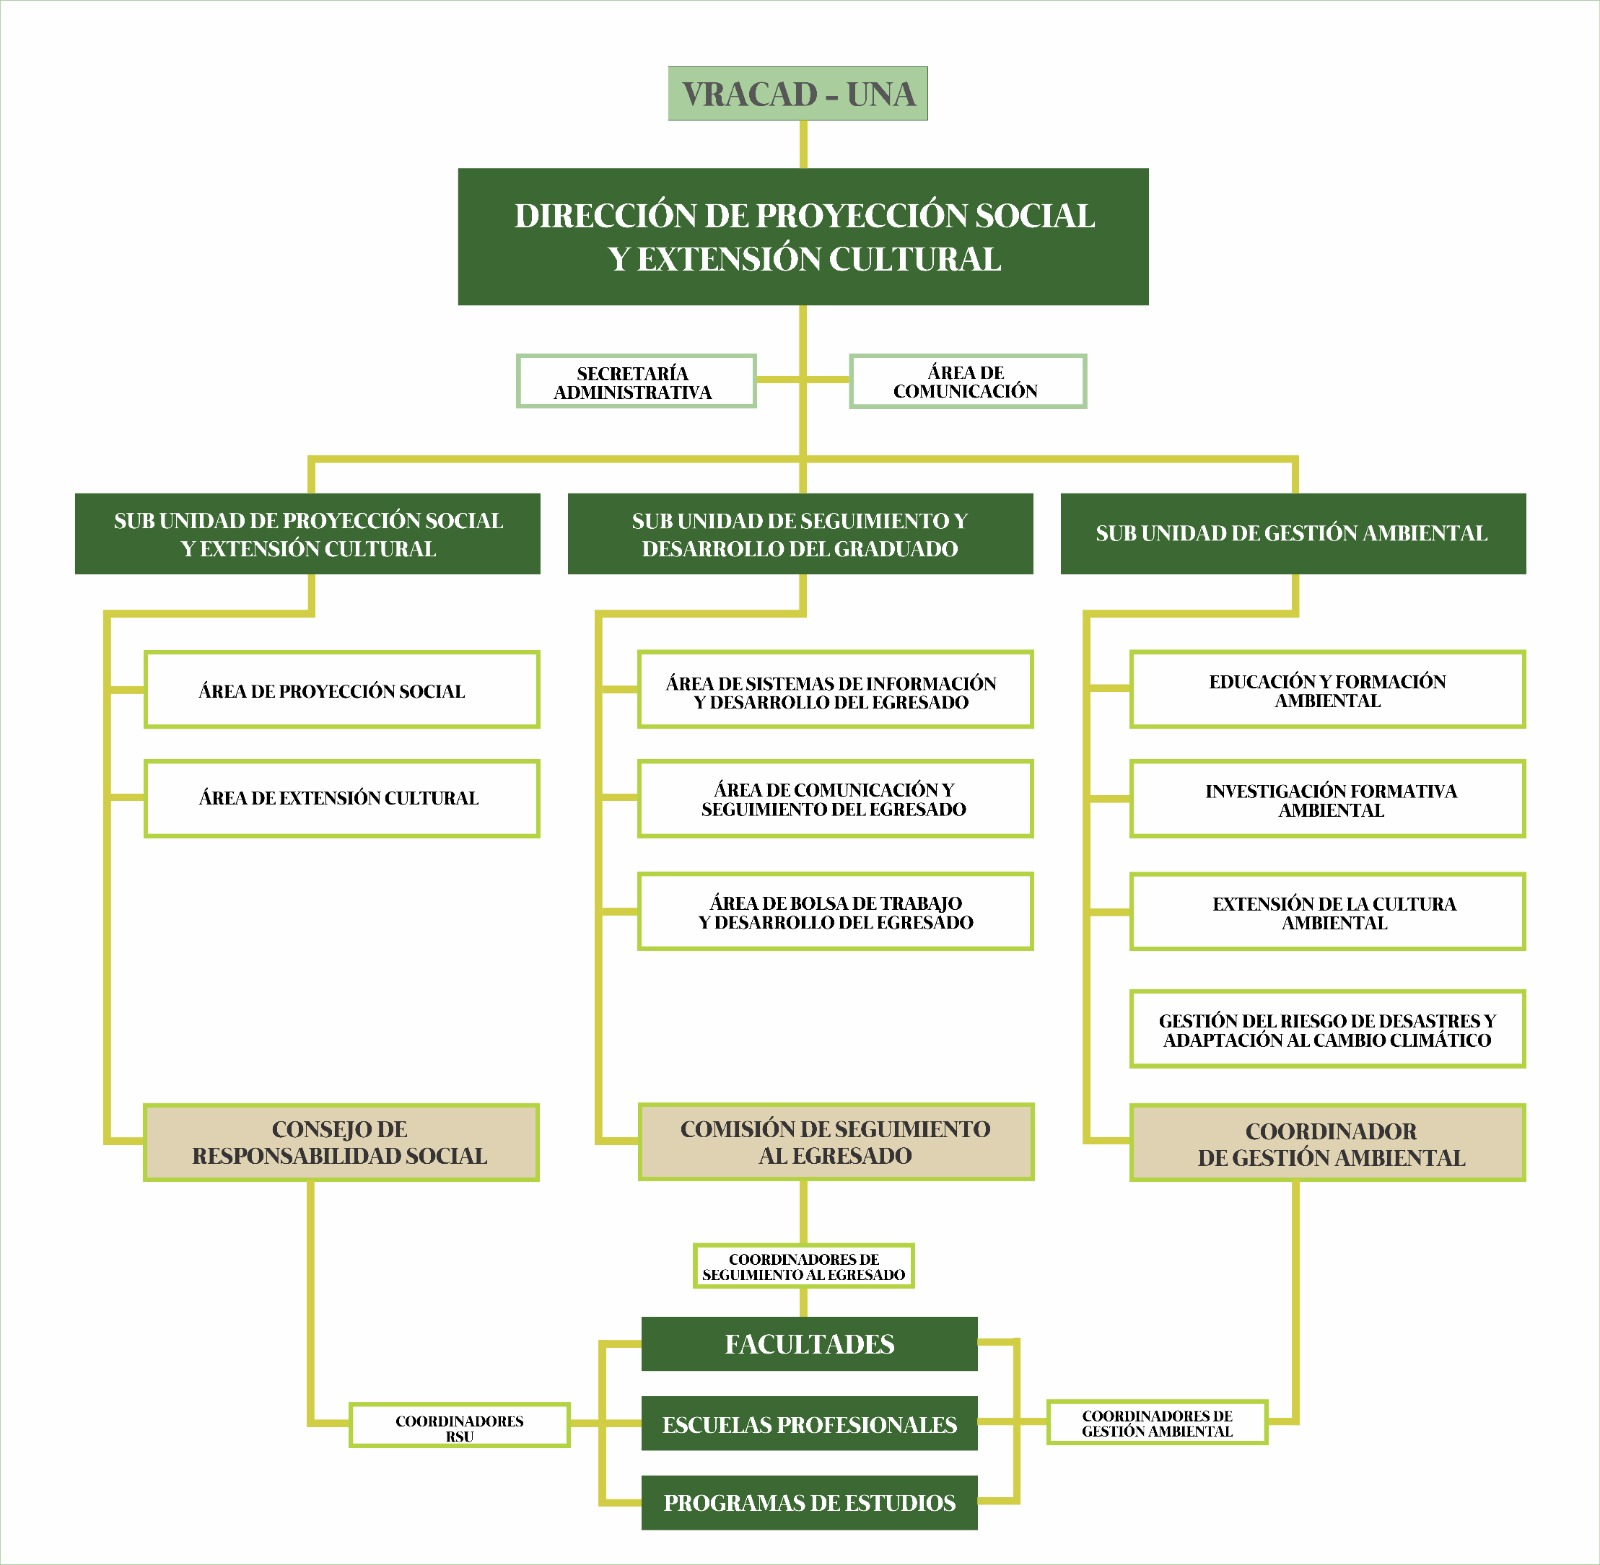
\includegraphics[width=0.8\textwidth]{images/estructura.jpeg} % Incluye la imagen y ajusta su ancho
    \label{fig:organigrama} % Etiqueta para referenciar
\end{figure}
\FloatBarrier
